\chapter{Introduction}
Nonlinear systems, as their name suggests, don't adhere to linear relationships between inputs and outputs. This lack of linearity means the system's response to input changes is intricate and often unpredictable. In the real world, nearly all systems exhibit some form of nonlinearity. This nonlinearity manifests in various phenomena. For instance, in systems with multiple inputs and multiple outputs, interdependencies between variables become complex, posing a coupling problem. Chaotic behavior, often referred to as the butterfly effect, is another common issue. Even a slight alteration in initial conditions can drastically alter the system's outcome. The classic butterfly effect example illustrates this sensitivity — a butterfly's wings in Brazil potentially triggering a tornado in Texas. When dealing with control tasks, especially in many real-world systems, accounting for this nonlinearity is essential.

Gaining proficient control over nonlinear systems has been a primary objective in the field of control theory for a substantial period. Throughout history, control engineers have developed a diverse range of approaches to handle these intricate systems. The advent of robotics in recent times has brought forth new methodologies specifically designed to tackle the challenges posed by nonlinearities.

\section{Motivation}
Robots, which are programmable mechanical entities, are purposefully designed for autonomous or semi-autonomous task execution, showcasing mobility, manipulation, and interaction with their surroundings.

In the realm of modern robotics, these machines exemplify intricate, highly nonlinear mechanical systems. Some well-known instances include quadruped robotics, autonomous vehicles, quadcopters, and humanoid robots.

\begin{figure}[!htbp]
  \centering
  \begin{minipage}[b]{0.40\textwidth}
    \centering
    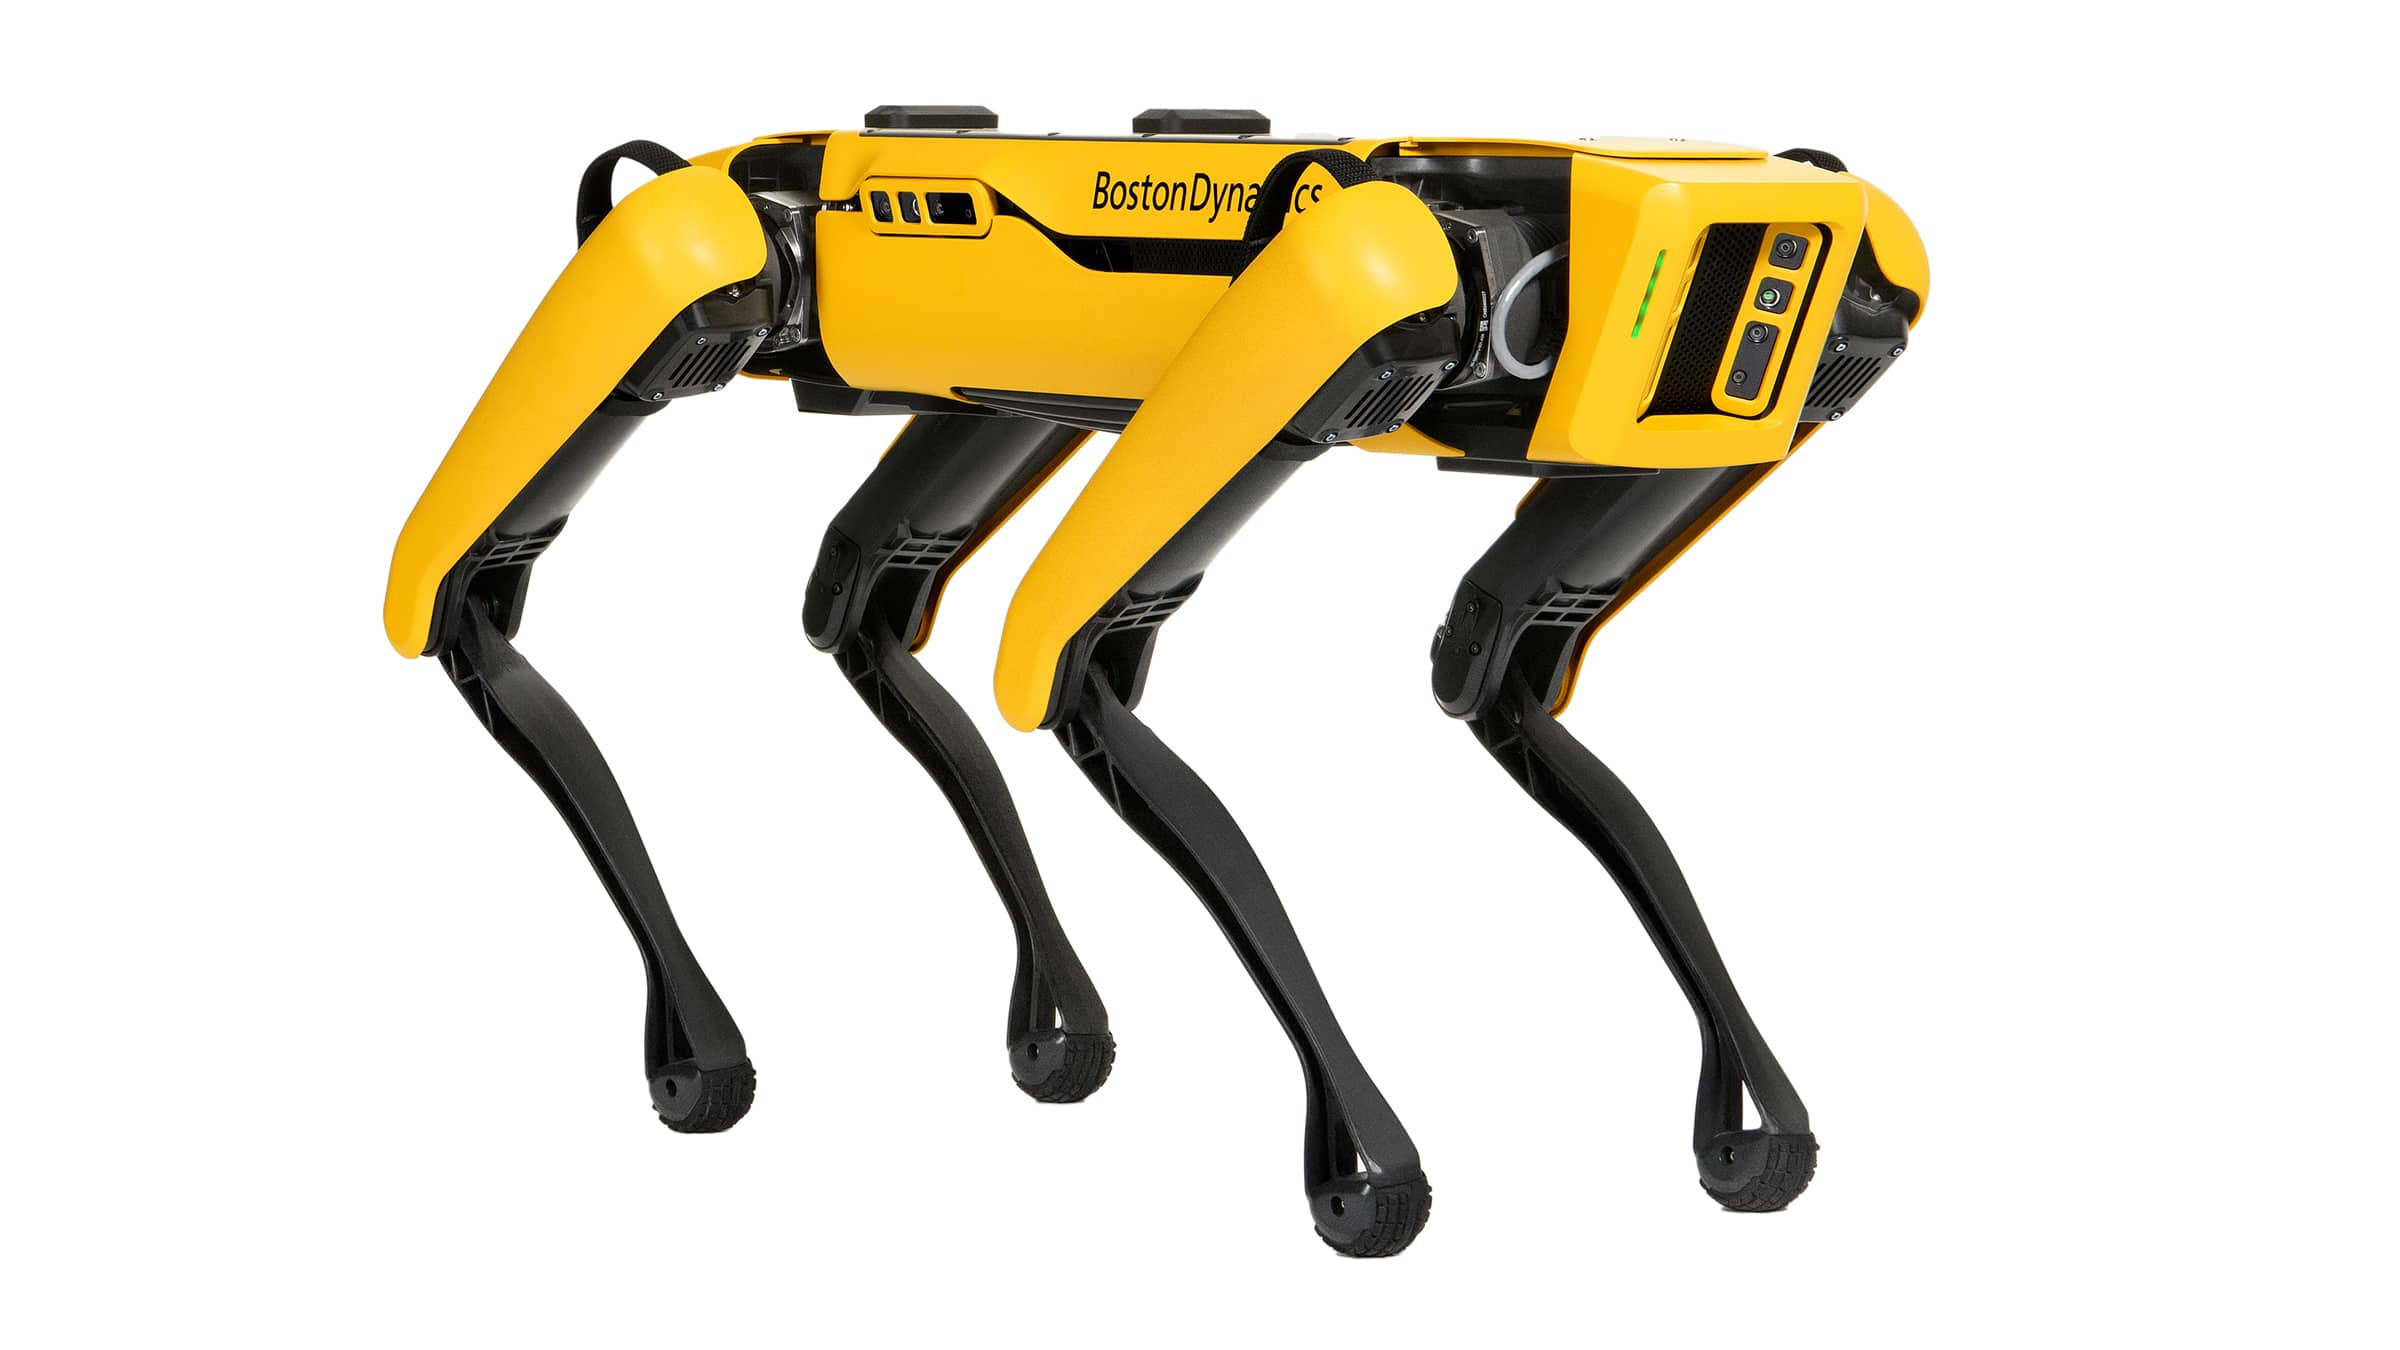
\includegraphics[width=\textwidth]{figures/quadruped.jpg}
    \caption{Caption for Image 1}
    \label{fig:image1}
  \end{minipage}
  \hfill
  \begin{minipage}[b]{0.40\textwidth}
    \centering
    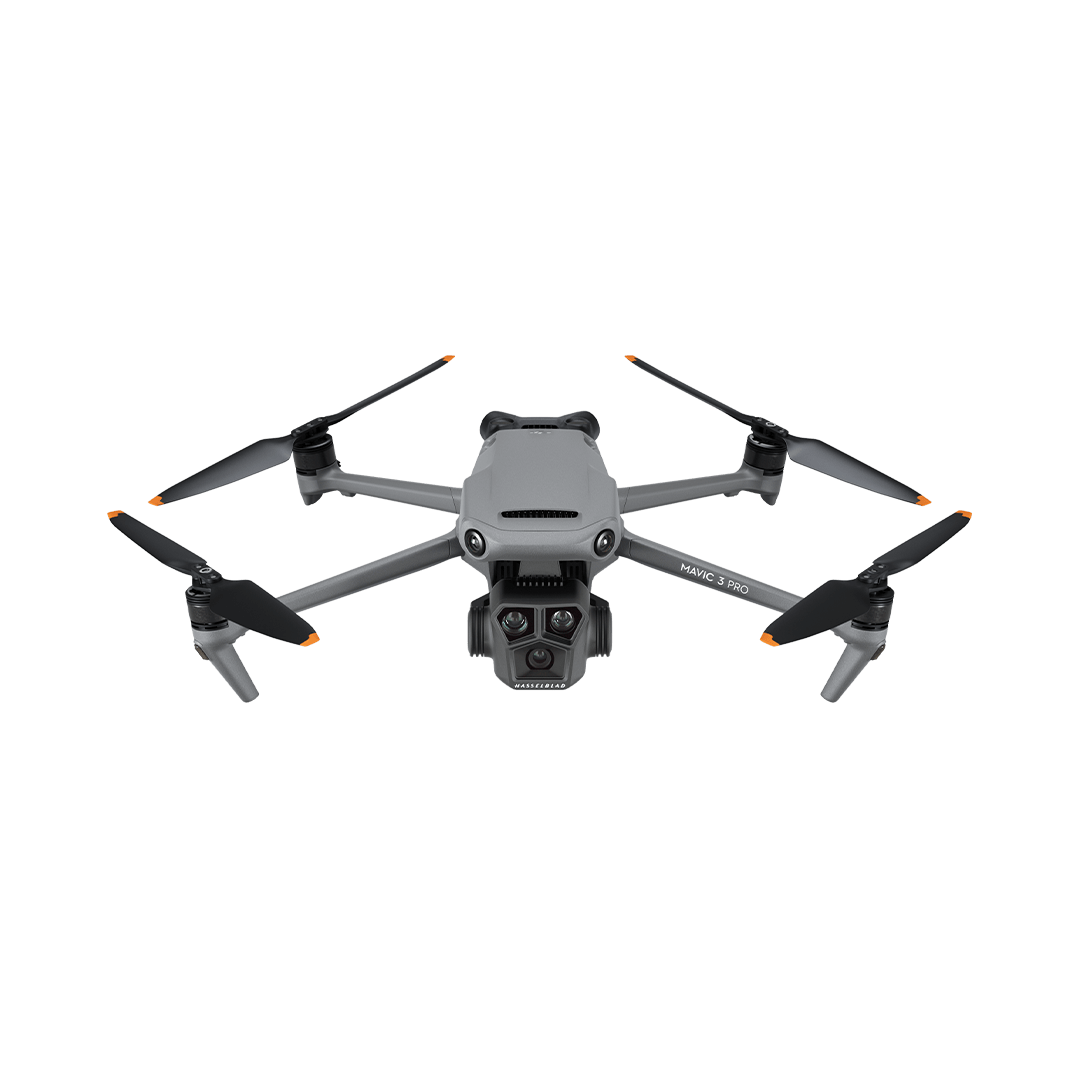
\includegraphics[width=\textwidth]{figures/quadcopter.png}
    \caption{Caption for Image 2}
    \label{fig:image2}
  \end{minipage}
  
  \vspace{1em} % Adjust the vertical space between rows

  \begin{minipage}[b]{0.40\textwidth}
    \centering
    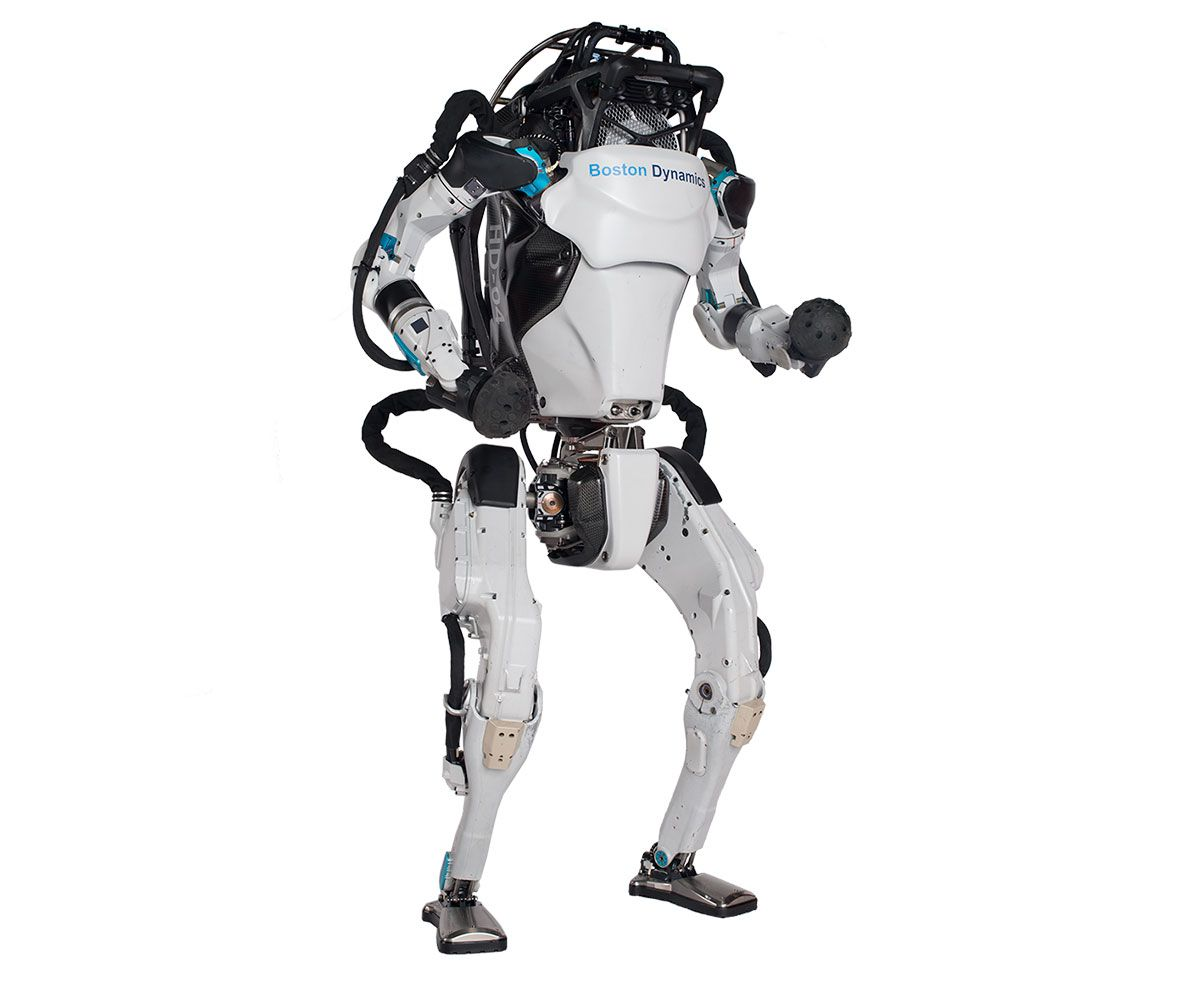
\includegraphics[width=\textwidth]{figures/humanoid.jpg}
    \caption{Caption for Image 3}
    \label{fig:image3}
  \end{minipage}
  \hfill
  \begin{minipage}[b]{0.40\textwidth}
    \centering
    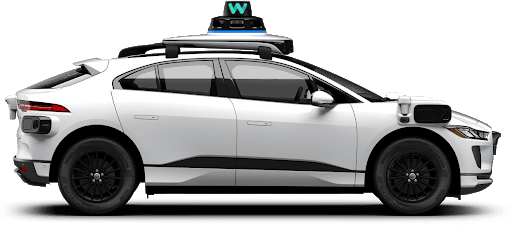
\includegraphics[width=\textwidth]{figures/waymo.png}
    \caption{Caption for Image 4}
    \label{fig:image4}
  \end{minipage}
\end{figure}

\subsection{Trajectory planning and tracking}
To enhance their motion capabilities, reliable nonlinear control methods are essential. Traditionally, for planning complex motion in systems like those mentioned above, a two-step approach is followed, namely trajectory planning and trajectory tracking.

Trajectory planning involves computing a smooth and feasible path that a robot should follow to reach a specific target position or work point. A common method employed is trajectory optimization, aiming to minimize a cost function that factors in travel time, energy consumption, and smoothness of motion. Techniques such as gradient descent or genetic algorithms are often used for this optimization. Adhering to constraints such as maximum velocity and accelerations is crucial during this process.

Once the trajectory is successfully planned, trajectory tracking involves implementing control algorithms to guide the robot along the planned trajectory. Typically, a feedback control approach is utilized, continuously monitoring the robot's position and adjusting control inputs. However, in real-world systems, even with a well-planned trajectory, external disturbances, uncertainties, or system limitations may cause significant deviations. Hence, accurate state estimation and robust control are crucial in the realm of feedback control.

[maybe there a better example is to explain how atlas works]
In the domain of industrial robot control, it's typical to separate the process into distinct planning and execution phases. This division arises from the fact that real-time responsiveness is not a stringent necessity in this context. When a task is defined, the planning phase kicks in, utilizing algorithms like linear interpolation and A* for trajectory generation. Following this, a steady and reliable control policy is implemented to ensure precise tracking of the generated trajectory during the execution phase.

Yet, in dynamic domains like automotive and flight control, the demand for real-time responsiveness takes center stage. Model Predictive Control (MPC) stands as a prime illustration of this critical requirement. MPC seamlessly integrates trajectory planning and execution into a unified framework. The process commences by projecting a sequence of control actions into the future as part of the planning stage. Subsequently, the calculated control inputs are meticulously fine-tuned to minimize the deviation between the actual system state and the planned trajectory. This strategic implementation effectively guides the system to closely track the intended trajectory.

MPC's brilliance lies in its ability to concurrently devise and optimize trajectories while swiftly adapting in real time to stay closely aligned with the planned trajectory, even when facing various disturbances and uncertainties. This amalgamation plays a pivotal role in achieving precise control and adaptability, especially in rapidly changing and intricate environments.

Though the traditional approach of trajectory generation and tracking has proven effective for many systems, it has the following drawbacks:
\begin{itemize}
    \item \textbf{Limited Adaptability:}
    Trajectory planning typically relies on predefined paths or trajectories, limiting adaptability to unforeseen changes or dynamic environments. If the environment changes significantly, the planned trajectory may no longer be optimal or even feasible.
    
    \item \textbf{Difficulty in Complex Environments:}
    In highly complex and cluttered environments, planning a feasible trajectory that avoids obstacles while reaching the goal can be challenging. The complexity increases with the number of obstacles and the intricacy of the environment.
    
    \item \textbf{Difficulty with Nonlinear Systems:}
    Trajectory planning struggles with highly nonlinear systems where the dynamics are hard to model accurately. Linearizing the system for planning purposes may lead to suboptimal or infeasible trajectories.
    
    \item \textbf{Static Planning:}
    Traditional trajectory planning is often static, assuming a stationary environment. It does not readily adapt to changing circumstances or dynamic obstacles, which limits its applicability in real-world scenarios.
    
    \item \textbf{High Computational Demands:}
    Some trajectory planning algorithms can be computationally intensive, especially for high-dimensional or complex robotic systems. This computational demand becomes a drawback, particularly in real-time or time-critical applications.
\end{itemize}

\subsection{Reinforcement learning based control}
In contrast to trajectory-based control, reinforcement learning (RL)-based control extracts an optimal policy through interactions with the environment, offering several advantages:

\begin{itemize}
    \item \textbf{Adaptability and Flexibility:}
    RL enables systems to adapt and learn optimal behavior in environments that are dynamic and chaning. The control policy can continuously evolve based on new experiences and acquired knowledge, ensuring adaptability to varying circumstances.
    
    \item \textbf{Less Model Information Required:}
    In contrast to traditional control methods that often necessitate a precise mathematical model of the system, RL can directly learn from interactions with the environment without relying on an explicit model. This characteristic is particularly valuable in scenarios where system dynamics are complex or unknown.
    
    \item \textbf{Effective Handling of Nonlinearities and Complex Systems:}
    RL proves highly effective in dealing with highly nonlinear systems and complex control tasks that might pose challenges for traditional control methods. The use of neural network-based function approximation allows for the capture of intricate relationships between states and actions.
    
    \item \textbf{Efficient Handling of High-Dimensional Input Spaces:}
    RL demonstrates an ability to efficiently manage high-dimensional and continuous input spaces, a crucial feature in many real-world applications such as robotics, finance, and game playing.
\end{itemize}

Reinforcement learning, by learning directly from the environment, offers a dynamic and adaptable approach to control, making it particularly suitable for complex and nonlinear systems.


\section{Problem setup}
Within the realm of nonlinear systems, a particularly challenging class is underactuated systems. These systems are characterized by having fewer control inputs than degrees of freedom. This makes them notably harder to control compared to fully actuated systems. Interestingly, a majority of robots and even living beings in nature fall into the category of underactuated systems. Consequently, studying the control of underactuated mechanical systems holds significant universal relevance.

The double pendulum, a simple setup comprising two links connected by two rotational joints, is a prime example. The joints involved are the shoulder joint, directly connected to the world frame, and the elbow joint, situated between the two links. The end effector is positioned at the tip of the second link. Active control is achieved by attaching motors to the shoulder and elbow joints. In the domain of underactuated control, if the shoulder joint is actuated, the setup is known as a pendubot. On the other hand, if the elbow joint is actuated, it's referred to as an acrobot.

\begin{figure}[h]
  \centering
  \includegraphics[width=0.5\textwidth]{example-image} % Replace "example-image" with the actual image file name and path
  \caption{This is a sample image.}
  \label{fig:sample}
\end{figure}

Despite its simple configuration, the system exhibits highly nonlinear and chaotic behavior. The double pendulum setup presents two classic tasks: swing-up and stabilization around the highest point. Research on swing-up and stabilization of the double pendulum can be traced back to the 1990s, and it continues to be a crucial testbed for validating the effectiveness of newly designed control algorithms.

Our project's motivation is to develop a reinforcement learning-based control method suitable for underactuated control of the double pendulum system, specifically addressing swing-up and stabilization tasks. To evaluate the efficacy of this control method, we conduct both simulations and real system experiments.


\section{Contribution}
In this paper, our main contribution is as follows: developing an effective control strategy to achieve two key objectives with the double pendulum. The first task involves swinging the double pendulum from its lowest point to its highest point. The second task is to maintain stability at the highest point. 

To tackle the swing-up task, we utilized a well-known model-free reinforcement learning algorithm called soft actor-critic. This algorithm allowed us to train a policy capable of reaching the region of attraction (RoA) of a continuous-time linear quadratic regulator (LQR) controller. Once the system enters the RoA, we seamlessly transition to the LQR controller to maintain stability around the highest point.

\section{Content}
The paper is structured as follows:

\begin{itemize}
  \item \textbf{Chapter 2: State-of-the-Art}
  \begin{itemize}
    \item This chapter provides an overview of current advancements in the field, summarizing essential theories, including those related to nonlinear and underactuated control.
  \end{itemize}
  
  \item \textbf{Chapter 3: Methodology}
  \begin{itemize}
    \item This chapter delves into the methodology, encompassing fundamental aspects of reinforcement learning, with a specific focus on the SAC algorithm. It explains the reward function used for training, the training procedure, and covers the concept of the LQR controller and how the combined controller was composed.
  \end{itemize}
  
  \item \textbf{Chapter 4: Simulation Results}
  \begin{itemize}
    \item In this chapter, we present the results obtained from simulations, showcasing the performance and behavior of the designed control strategy.
  \end{itemize}
  
  \item \textbf{Chapter 5: Hardware Results}
  \begin{itemize}
    \item This chapter reports the outcomes of experiments conducted on the hardware, providing insights into how we addressed the sim2real transfer problem.
  \end{itemize}
  
  \item \textbf{Chapter 6: Discussion and Future Work}
  \begin{itemize}
    \item The final chapter engages in a discussion about the obtained results and explores potential future directions for research and development.
  \end{itemize}
\end{itemize}

\cleardoublepage
